% --------------------------------------------------------------
%                         Preamble
% --------------------------------------------------------------

\documentclass[12pt, letter]{article}
\usepackage[latin1]{inputenc}
\usepackage[T1]{fontenc}
\usepackage{amsmath,amssymb,amsthm}
\usepackage{longtable}
\usepackage{enumitem}
\usepackage{hyperref}
\usepackage{verbatim}
\usepackage{bm}
\usepackage[framemethod=tikz]{mdframed}
\usepackage{graphicx}
\usepackage{amsmath}
\hypersetup{
    colorlinks=true,
    linkcolor=blue,
    filecolor=magenta,      
    urlcolor=blue,
}
 
\urlstyle{same}

\usepackage{array}
\newcolumntype{L}[1]{>{\raggedright\let\newline\\\arraybackslash\hspace{0pt}}m{#1}}
\newcolumntype{C}[1]{>{\centering\let\newline\\\arraybackslash\hspace{0pt}}m{#1}}
\newcolumntype{R}[1]{>{\raggedleft\let\newline\\\arraybackslash\hspace{0pt}}m{#1}}
\newcommand{\norm}[1]{\left\lVert#1\right\rVert}
\newcommand{\vs}[1][1]{\vspace{#1\baselineskip}}

\DeclareMathOperator{\depth}{depth}
\DeclareMathOperator{\im}{im}
\DeclareMathOperator{\coker}{coker}
\DeclareMathOperator{\rank}{rank}
\DeclareMathOperator{\Proj}{Proj}
\DeclareMathOperator{\Hom}{Hom}
\DeclareMathOperator{\Tor}{Tor}
\DeclareMathOperator{\Ext}{Ext}
\DeclareMathOperator{\HH}{H}

% page format

\topmargin -15mm \textwidth 168mm \textheight 240mm \oddsidemargin
-8mm \evensidemargin 0mm
\setlength{\parindent}{0pt}

% some environments :

\theoremstyle{plain}
\newtheorem{theorem}{Theorem}
\newtheorem{lemma}[theorem]{Lemma}
\newtheorem{corollary}[theorem]{Corollary}
\newtheorem{proposition}[theorem]{Proposition}

\numberwithin{theorem}{section}

\theoremstyle{definition}
\newtheorem{definition}[theorem]{Definition}
\newtheorem{example}[theorem]{Example}
\newtheorem{problem}[theorem]{Problem}
\newtheorem{exercise}[theorem]{Exercise}
\newtheorem{algorithm}[theorem]{Algorithm}
\newtheorem{note}[theorem]{Note}
\newtheorem{remark}[theorem]{Remark}
\newtheorem{question}[theorem]{Question}

% using AMS mathematical symbols

\usepackage{latexsym}            % for the qed symbol
\usepackage{amssymb}

\newcommand{\N}{\mathbb{N}}
\newcommand{\Z}{\mathbb{Z}}
\newcommand{\Q}{\mathbb{Q}}
\newcommand{\R}{\mathbb{R}}

\def\qex{\hfill \quad\vrule height1.2ex width0.5em depth 0pt} % end of example


\begin{document}

% --------------------------------------------------------------
%                         Start here
% --------------------------------------------------------------

\noindent
Colorado State University \hfill Section 5 (4:00-4:50pm)\\
Department of Mathematics\ \  \hfill  Math 261, Fall 2019\\
\bigskip
\thispagestyle{empty}

\begin{center}
\begin{large}
\textbf{Lecture Notes-Midterm 1\\
}
\end{large}
\end{center}

% --------------------------------------------------------------
%                         Intro
% --------------------------------------------------------------

\noindent These notes were created by Scott Ziegler for Math 261 at Colorado State University and adapted from Thomas' Calculus, 13th Edition, Pearson Education Inc, 2010. The listed section numbers correspond to the sections of the aforementioned text.


% --------------------------------------------------------------
%                         Sec 12.1
% --------------------------------------------------------------

\section{Three-Dimensional Coordinate Systems (12.1)}

\begin{itemize}
\item In Calc I and II, we learned a good deal about functions over one dimension. The focus of this class will be adapting what we learned in Calc I and II to higher dimensions, particularly three dimensions.
\item We'll start this process by drawing three dimensional cartesian space and defining a few things.
\end{itemize}

\hrulefill

\begin{center}
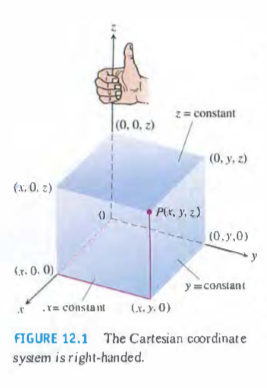
\includegraphics[scale=0.8]{m1_f1}
\end{center}

\bigskip

\begin{definition}
The above drawing depicts the three dimensional \textbf{cartesian coordinate system}. Cartesian coordinates are also called \textbf{rectangular coordinates} because the axes that define them meet at right angles.
\end{definition}

\bigskip

\begin{definition}
\begin{itemize}
\item The planes determined by the coordinate axes are the \textbf{xy-plane}, whose standard equation is $z=0$; the \textbf{yz-plane}, whose standard equation is $x=0$; and the \textbf{xz-plane}, whose standard equation is $y=0$.
\item The three planes determined by the coordinate axes meet at the \textbf{origin} $(0,0,0)$. We will often denote the origin by $0$ or $\mathcal{O}$.
\end{itemize}
\end{definition}

\bigskip

\begin{definition}
The three coordinate planes ($x=0, \ y=0, \ z=0$) divide space into eight cells which we call \textbf{octants}. The octant in which the point coordinates are all positive is called the \textbf{first octant}.
\end{definition}

\bigskip

\textbf{Notes:}
\begin{itemize}
\item There is no convention for labeling the other seven octants.
\item We say that the coordinate system above is \textit{right-handed}. When we curl the fingers of our right hand from the positive x-axis to the positive y-axis, our thumb points up in the direction of the positive z-axis.
\item We denote an arbitrary point in three dimensional cartesian space by $P(x,y,z)$.
\end{itemize}

\bigskip

\hrulefill

\bigskip

\begin{example}
Plot the points $(1,1,1)$, $(-1,1,2)$, $(2,0,0)$.
\end{example}

\bigskip

\hrulefill

\bigskip

\begin{example}
Sketch the planes given by the equations $x=3$, $y=1$. What can we say about the intersection of these two planes? Now also sketch the plane given by the equation $z=2$. What can we say about the intersection of these three planes?
\end{example}

\bigskip

\hrulefill

\bigskip

\begin{example}
Interpret the following equations and inequalities geometrically.
\begin{itemize}
\item $z \geq 0$. The half-space consisting of points on and above the xy-plane.
\item $x=-3$. The plane perpendicular to the x-axis at $x=-3$.
\item $z=0, \ x\leq 0, \ y \geq 0$. The second quadrant of the xy-plane.
\item $x \geq 0, y \geq 0, z \geq 0$. The first octant.
\item $-1 \leq y \leq 1$. The slab (or if you want, infinite rectangular prism) between and including the planes $y=-1$ and $y=1$.
\item $y=-2, z=2$. The line in which the planes $y=-2$ and $z=2$ intersect.
\end{itemize}
\end{example}

\bigskip

\hrulefill

\bigskip

\begin{example}
What points $P(x,y,z)$ satisfy the equations
\begin{align*}
x^2+y^2=4 \ \ \ \ \text{and} \ \ \ \ z=3?
\end{align*}
These are the points lying in the horizontal plane $z=3$, on the circle given by $x^2+y^2=4$. We could call this set of points ``the circle $x^2+y^2=4$ in the plane $z=3$".
\end{example}

\bigskip

\hrulefill

\bigskip

\subsection{Distance and Spheres in Space}
The formula for distance between two points in two dimensions (the xy-plane) extends to points in three dimensions.

\bigskip

\begin{definition}
The \textbf{distance} between two points $P_1(x_1,y_1,z_1)$ and $P_2(x_2,y_2,z_2)$ is given by
\begin{align*}
|P_1P_2| = \sqrt{(x_2-x_1)^2+(y_2-y_1)^2+(z_2-z_1)^2}
\end{align*}
\end{definition}

\bigskip

\hrulefill

\bigskip

\begin{example}
Find the distance between the points $P_1(2,1,5)$ and $P_2(-2,3,0)$.\\

\smallskip

We can use the above formula to find
\begin{align*}
|P_1P_2| &= \sqrt{(-2-2)^2+(3-1)^2+(0-5)^2}\\
&= \sqrt{16+4+25}\\
&=\sqrt{45}.
\end{align*}
\end{example}

\bigskip

\hrulefill

\bigskip

\begin{definition}
The \textbf{standard equation for the sphere} of radius $a$ and center $(x_0,y_0,z_0)$ is given by
\begin{align*}
(x-x_0)^2+(y-y_0)^2+(z-z_0)^2=a^2.
\end{align*}
\end{definition}

\bigskip

\hrulefill

\bigskip

\begin{example}
Find the center and radius of the sphere
\begin{align*}
x^2+y^2+z^2+3x-4z+1=0.
\end{align*}
We'll proceed by completing the square for the $x, \ y$ and $z$ terms, writing each quadratic as a squared linear expression, then reading off the center and radius of the equation in standard form.
\begin{align*}
x^2+y^2+&z^2+3x-4z+1=0 \Rightarrow (x^2+3x)+y^2+(z^2-4z) = -1\\
&\Rightarrow \left(x^2+3x+\left(\frac{3}{2}\right)^2\right) + y^2 + \left(z^2-4z+\left(\frac{-4}{2}\right)^2\right) = -1+\left(\frac{3}{2}\right)^2+\left(\frac{-4}{2}\right)^2\\
&\Rightarrow \left(x+\frac{3}{2}\right)^2+y^2+(z-2)^2 = \frac{21}{4}.
\end{align*}
We can now read off that the center is $\left(-\frac{3}{2},0,2\right)$ with center $\frac{\sqrt{21}}{2}$.
\end{example}

\bigskip

\hrulefill

\bigskip

\begin{example}
Interpret the following equations and inequalities geometrically.
\begin{itemize}
\item $x^2+y^2+z^2<4$. The interior of the sphere $x^2+y^2+z^2=4$.
\item $x^2+y^2+z^2\leq4$. The solid ball give by the sphere $x^2+y^2+z^2=4$ and its interior.
\item $x^2+y^2+z^2>4$ The exterior of the sphere $x^2+y^2+z^2=4$.
\item $x^2+y^2+z^2=4, \ z\leq 0$. The lower half of the sphere $x^2+y^2+z^2=4$.
\end{itemize}
\end{example}

\newpage

% --------------------------------------------------------------
%                         Sec 12.2
% --------------------------------------------------------------

\section{Vectors (12.2)}

The concept of a vector is very important. Unfortunately, there is a bit of ambiguity to the term ``vector" due to people in different fields of study viewing this concept differently. Mathematicians, physicists, and computer scientists all think of different things when they hear the word vector. We will be thinking of vectors in this class primarily in the same way that physicists do, which is actually just a specific case of the way mathematicians view vectors. We will unequivocally \textit{not} think of vectors the way that computer scientists think of them.

\bigskip

\hrulefill

\bigskip

\begin{definition}
A \textbf{vector} is an object having both magnitude and direction. When possible, vectors are represented by a \textbf{directed line segment}.
\end{definition}

\bigskip

\begin{center}
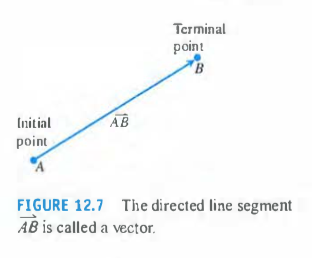
\includegraphics[scale=0.7]{m1_f2}
\end{center}

\bigskip

\textbf{Notes:}
\begin{itemize}
\item Examples of vectors you may have seen are force, displacement, and velocity.
\item We denote a vector by $\bm{v}$ or $\vec{v}$.
\end{itemize}

\bigskip

\hrulefill

\bigskip

\begin{definition}
The vector represented by the directed line segment $\vec{AB}$ has \textbf{initial point} A and \textbf{terminal point} B and its \textbf{length} is denoted by $|\vec{AB}|$. Two vectors are \textbf{equal} if they have the same length and direction.
\end{definition}

\bigskip

\begin{center}
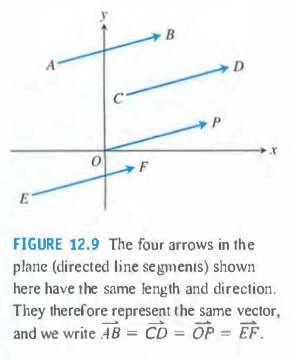
\includegraphics[scale=0.7]{m1_f3}
\end{center}

\bigskip

\textbf{Note:} A vector whose initial point is the origin is said to be in \textbf{standard form}. When a vector is in standard form, it can be completely described by its terminal point.

\bigskip

\hrulefill

\bigskip

If we are dealing with a two or three-dimensional vector, we typically represent the vector in what is known as component form.

\bigskip

\begin{definition}
If $\bm{v}$ is a two-dimensional vector in the plane equal to the vector with initial point at the origin and the terminal point $(v_1,v_2)$, then the \textbf{component form} of $\bm{v}$ is
\begin{align*}
\bm{v} = \langle v_1, v_2 \rangle.
\end{align*}
If $\bm{v}$ is a three-dimensional vector equal to the vector with initial point at the origin and the terminal point $(v_1,v_2,v_3)$, then the \textbf{component form} of $\bm{v}$ is
\begin{align*}
\bm{v} = \langle v_1, v_2, v_3 \rangle.
\end{align*}
\end{definition}

\bigskip

\textbf{Notes:}
\begin{itemize}
\item The numbers $v_1, v_2, v_3$ are called the \textbf{components} of the vector $\bm{v}$.
\item Two vectors $u=\langle u_1,u_2,u_3 \rangle$ and $v= \langle v_1,v_2,v_3\rangle$ are equal if and only if $u_1=v_1$, $u_2=v_2$, $u_3=v_3$.
\item If a vector is not in standard form, that is a vector $\bm{v}$ with initial point $P(x_1,y_1,z_1)$ and terminal point $Q(x_2,y_2,z_2)$ can be represented in standard form as $\bm{v} = \langle x_2-x_1, y_2-y_2, z_2-z_1 \rangle$.
\end{itemize}

\bigskip

\hrulefill

\bigskip

\begin{definition}
The \textbf{magnitude} or \textbf{length} of the vector $\bm{v} = \vec{PQ}$ is the nonnegative number
\begin{align*}
|\bm{v}| = ||\bm{v}|| = \sqrt{v_1^2+v_2^2+v_3^2} = \sqrt{(x_2-x_1)^2+(y_2-y_1)^2+(z_2-z_1)^2}.
\end{align*}
\end{definition}

\bigskip

The only vector with length zero is called the \textbf{zero vector} $\bm{0} = \langle 0, 0 \rangle$ or $\bm{0} = \langle 0, 0 ,0 \rangle$.

\bigskip

\hrulefill

\bigskip

\begin{example}
Find the component form and length of the vector $\bm{v} = \vec{PQ}$ with initial point $P(-3,4,1)$ and terminal point $Q(-5,2,2)$.\\

\smallskip

We have
\begin{align*}
v_1 &= x_2-x_1 = -5-(-3) = -2\\
v_2 &= y_2-y_1 = 2-4 = -2\\
v_3 &= z_2-z_1 = 2-1 = 1.
\end{align*}
So the component form of this vector is $\bm{v} = \langle -2, -2, 1 \rangle$. The magnitude of this vector is
\begin{align*}
||\bm{v}|| = \sqrt{(-2)^2+(-2)^2+1^2} = \sqrt{9} = 3.
\end{align*}
\end{example}

\bigskip

\hrulefill

\bigskip

Now that we have defined and seen notation for vectors, the next natural step is to wonder what we can do algebraically with them. Can we add them? Multiply them? Divide them? We'll answer some of these in time, but for now we'll just look at two principal operations involving vectors called \textit{vector addition} and \textit{scalar multiplication}. For the purposes of this class, a \textbf{scalar} will just be a real number.

\bigskip

\begin{definition}
Let $\bm{u} = \langle u_1,u_2,u_3 \rangle$ and $\bm{v} = \langle v_1, v_2, v_3 \rangle$ be vectors and let $k$ be a scalar.\\
\begin{align*}
\textbf{Addition:} \ \ \ \ \ \ \ &\bm{u}+\bm{v} = \langle u_1+v_1, u_2+v_2, u_3+v_3 \rangle\\
\textbf{Scalar multiplication:} \ \ \ \ \ \ &k\bm{u} = \langle ku_1, ku_2, ku_3 \rangle.
\end{align*}
\end{definition}

\bigskip

\textbf{Notes:} 
\begin{itemize}
\item Subtracting the vectors $\bm{u}$ and $\bm{v}$ is the same as adding the vectors $\bm{u}$ and $-\bm{v}$.
\item The above definition is how mathematicians typically think of a vector.
\end{itemize}

\bigskip

\begin{center}
  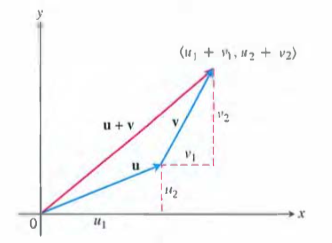
\includegraphics[scale = 0.5]{m1_f4}
  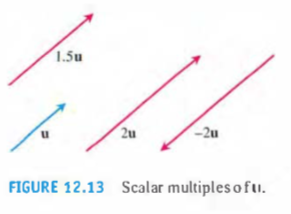
\includegraphics[scale = 0.5]{m1_f5}
\end{center}

\bigskip

\hrulefill

\bigskip

\begin{example}
Let $\bm{u} = \langle -1, 3, 1 \rangle$ and $\bm{v} = \langle 4, 7, 0 \rangle$. Find the components of
\begin{itemize}
\item $2\bm{u}+ 3\bm{v}$\\
\begin{align*}
2\bm{u}+3\bm{v} &= 2\langle -1, 3, 1 \rangle+3\langle 4, 7, 0 \rangle\\
&= \langle -2, 6, 2 \rangle + \langle 12, 21, 0 \rangle\\
&= \langle 10, 27, 2 \rangle
\end{align*}
\item $\bm{u}-\bm{v}$
\begin{align*}
\bm{u}-\bm{v} &= \bm{u}+(-\bm{v})\\
&= \langle -1,3,1 \rangle + \langle -4, -7, 0 \rangle\\
&= \langle -5, -4, 1 \rangle
\end{align*}
\item $\left\Vert\frac{1}{2} \bm{u}\right\Vert$
\begin{align*}
\left\Vert\frac{1}{2} \bm{u}\right\Vert &= \left\Vert \langle -\frac{1}{2},\frac{3}{2},\frac{1}{2}\rangle \right\Vert\\
&= \sqrt{\left(-\frac{1}{2}\right)^2+\left(\frac{3}{2}\right)^2+\left(\frac{1}{2}\right)^2}\\
&= \frac{1}{2} \sqrt{11}
\end{align*}
\end{itemize}
\end{example}

\bigskip

\hrulefill

\bigskip

\begin{definition}
A vector $\bm{v}$ of length 1 is called a \textbf{unit vector}. The \textbf{standard unit vectors} are
\begin{align*}
\bm{i} = \langle 1, 0, 0 \rangle \ \ \ \bm{j} = \langle 0, 1, 0 \rangle \ \ \ \bm{k} = \langle 0, 0, 1 \rangle.
\end{align*}
\end{definition}

\bigskip

The vectors $\bm{i}, \bm{j}, \bm{k}$ above are also known as the \textbf{standard basis vectors} of $\R^3$. This is because any vector in three dimensional space can be written as a linear combination of these vectors. That is,
\begin{align*}
\bm{v} &= \langle v_1, v_2, v_3 \rangle\\
&= v_1 \bm{i} + v_2 \bm{j} + v_3 \bm{k}.
\end{align*}

\bigskip

\hrulefill

\bigskip

\begin{definition}
If $\bm{v} \neq \bm{0}$, then
\begin{itemize}
\item $\frac{\bm{v}}{||\bm{v}||}$ is a unit vector in the direction of $\bm{v}$.
\item The equation $\bm{v} = ||\bm{v}|| \frac{\bm{v}}{||\bm{v}||}$ expresses $\bm{v}$ as its length times its direction.
\end{itemize}
\end{definition}

\bigskip

\hrulefill

\bigskip

\begin{example}
Find a unit vector pointing in the direction of the vector from $P(1,0,1)$ to $Q(3,2,0)$.\\

\smallskip

Let $\bm{u}$ be the unit vector we want, then
\begin{align*}
\bm{u} &= \frac{\vec{PQ}}{||\vec{PQ}||}\\
&= \frac{\langle 3-1, 2-0, 0-1 \rangle}{\sqrt{(3-1)^2+(2-0)^2+(0-1)^2}}\\
&= \frac{\langle 2, 2, -1 \rangle} {3}\\
&= \left\langle \frac{2}{3}, \frac{2}{3}, -\frac{1}{3} \right\rangle.
\end{align*}
\end{example}

\bigskip

\hrulefill

\bigskip

\begin{example}
Rewrite $\vec{PQ}$ from the previous example as a product of its magnitude times its direction.\\

\smallskip

We found the direction $\frac{\vec{PQ}}{||\vec{PQ}||}$ in the last step, and in doing so we also calculated the magnitude $||\vec{PQ}||$. Thus we have
\begin{align*}
\vec{PQ} &= ||\vec{PQ}|| \frac{\vec{PQ}}{||\vec{PQ}||}\\
&= 3\left\langle \frac{2}{3}, \frac{2}{3}, -\frac{1}{3} \right\rangle\\
&= 3\left( \frac{2}{3}\bm{i}+ \frac{2}{3}\bm{j} -\frac{1}{3}\bm{k} \right).
\end{align*}
\end{example}

\newpage

% --------------------------------------------------------------
%                         Sec 12.3
% --------------------------------------------------------------

\section{The Dot Product (12.3)}

Suppose we have two vectors $\bm{u}$ and $\bm{v}$ in either two or three dimensions (this also generalizes to higher dimensions). There are times when it is useful for us to determine the angle $\theta$ between these vectors.

\bigskip

\begin{center}
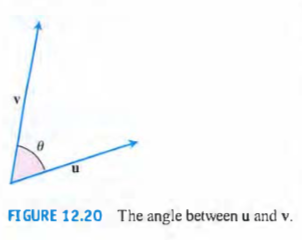
\includegraphics[scale=0.8]{m1_f6}
\end{center}

\bigskip

\hrulefill

\bigskip

\begin{theorem}{(\emph{Angle Between Two Vectors})}
The angle $\theta$ between two nonzero vectors $\bm{u} = \langle u_1, u_2, u_3 \rangle$ and $\bm{v} = \langle v_1, v_2, v_3 \rangle$ is given by
\begin{align*}
\theta = \arccos\left(\frac{u_1v_1+u_2v_2+u_3v_3}{||\bm{u}|| \ ||\bm{v}||}\right).
\end{align*}
\end{theorem}

\bigskip

\hrulefill

\bigskip

We will not prove this Theorem, but we could without too much trouble. The idea is to construct the following triangle:

\bigskip

\begin{center}
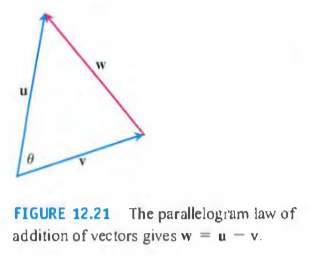
\includegraphics[scale=0.8]{m1_f7}
\end{center}

\bigskip

so that $\bm{w}=\bm{u}-\bm{v}$. We then use the law of cosines, cancel some things, move some things around and we have it. You're encouraged to try this an an exercise.

\bigskip

\hrulefill

\bigskip

Let's now focus on a particular expression in our previous theorem.

\bigskip

\begin{definition}
The \textbf{dot product} or \textbf{inner product}, denoted $\bm{u} \cdot \bm{v}$ (``$\bm{u}$ dot $\bm{v}$") of vectors $\bm{u} = \langle u_1, u_2, u_3 \rangle$ and $\bm{v} = \langle v_1, v_2, v_3 \rangle$ is
\begin{align*}
\bm{u} \cdot \bm{v} = u_1v_1 + u_2v_2 + u_3v_3.
\end{align*}
\end{definition}

\bigskip

\textbf{Notes:}
\begin{itemize}
\item We could equivalently write the dot product as $\bm{u}\cdot\bm{v} = ||\bm{u}||||\bm{v}||\cos(\theta)$.
\item The dot product of two vectors produces a scalar.
\item We'll see this dot product come up a lot in this course, which is why we're defining it. However it is also an example of an \textbf{inner product}, which you'll learn about more in linear algebra.
\item With the dot product, we can rewrite the expression for $\theta$ above as
\begin{align*}
\theta = \arccos\left(\frac{\bm{u}\cdot\bm{v}}{||\bm{u}|| \ ||\bm{v}||}\right).
\end{align*}
\end{itemize}

\bigskip

A couple of useful properties of the dot product:
\begin{itemize}
\item $\bm{u} \cdot \bm{v} = \bm{v} \cdot \bm{u}$
\item $\bm{u} \cdot (\bm{v}+\bm{w}) = \bm{u} \cdot \bm{v} + \bm{u} \cdot \bm{w}$
\item $\bm{u} \cdot \bm{0} = \bm{0}$
\end{itemize}

\bigskip

\hrulefill

\bigskip

\begin{example}
\begin{align*}
\langle 1, -2, -1 \rangle \cdot \langle -6, 2, -3 \rangle &= (1)(-6) + (-2)(2) + (-1)(-3)\\
& = -6-4+3\\
&= -7.
\end{align*}
\end{example}

\bigskip

\hrulefill

\bigskip

\begin{example}
Find the angle between $\bm{u} = \bm{i} - 2\bm{j} - 2\bm{k}$ and $\bm{v} = 6\bm{i}+3\bm{j}+2\bm{k}$.\\

\smallskip

Using our formula, we know that we must calculate the dot product of $\bm{u}$ and $\bm{v}$ as well as the magnitude (or norm) of each of the vectors.
\begin{align*}
\bm{u}\cdot\bm{v} &= (1)(6)+(-2)(3)+(-2)(2) = 6-6-4 = -4\\
||\bm{u}|| &= \sqrt{(1)^2+(-2)^2+(-2)^2} = \sqrt{9} = 3\\
||\bm{v}|| &= \sqrt{(6)^2+(3)^2+(2)^2} = \sqrt{49} = 7.
\end{align*}
Therefore we have
\begin{align*}
\theta &= \arccos\left(\frac{\bm{u}\cdot\bm{v}}{||\bm{u}|| \ ||\bm{v}||}\right)\\
&= \arccos\left(\frac{-4}{(3)(7)}\right)\\
&= \arccos\left(-\frac{4}{21}\right).
\end{align*}
\end{example}

\bigskip

\hrulefill

\bigskip

\begin{example}
Find the angle $\theta$ in the triangle $ABC$ determined by the vertices $A=(0,0), B = (3,5), C=(5,2)$.

\bigskip

\begin{center}
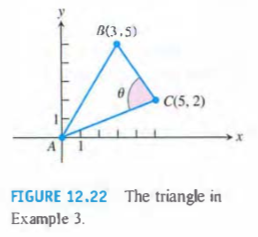
\includegraphics[scale=0.8]{m1_f8}
\end{center}

\bigskip
The angle $\theta$ is between the vectors $\vec{CA}$ and $\vec{CB}$, so we need the component form of these vectors. We get
\begin{align*}
\vec{CA} &= \langle 0-5, 0-2 \rangle = \langle -5, -2 \rangle\\
\vec{CB} &= \langle 3-5, 5-2 \rangle = \langle -2, 3 \rangle.
\end{align*}
Now we just need to find the dot product and magnitude of these vectors and plug it into our formula.
\begin{align*}
\vec{CA} \cdot \vec{CB} &= (-5)(-2)+(-2)(3) = 4\\
||\vec{CA}|| &= \sqrt{(-5)^2+(-2)^2} = \sqrt{29}\\
||\vec{CB}|| &= \sqrt{(-2)^2+(3)^2} = \sqrt{13}.
\end{align*}
We get
\begin{align*}
\theta &= \arccos\left(\frac{\vec{CA} \cdot \vec{CB}}{||\vec{CA}|| ||\vec{CB}||}\right)\\
&= \arccos\left(\frac{4}{\sqrt{29}\sqrt{13}}\right)\\
&\approx 1.36 \ \text{rad}.
\end{align*}
\end{example}

\bigskip

\hrulefill

\bigskip

\begin{definition}
Two vectors $\bm{u}$ and $\bm{v}$ are perpendicular or \textbf{orthogonal} is the angle between them is $\frac{\pi}{2}$. Equivalently, we say that the vectors $\bm{u}$ and $\bm{v}$ are \textbf{orthogonal} if and only if $\bm{u}\cdot\bm{v} = 0$.
\end{definition}

\bigskip

\hrulefill

\bigskip

\begin{example}
\begin{itemize}
\item[(a.)] $\bm{u} = \langle 3, -2 \rangle$ and $\bm{v} = \langle 4, 6 \rangle$ are orthogonal because $\bm{u} \cdot \bm{v} = (3)(4) + (-2)(6) = 0$.
\item[(b.)] $\bm{u} = \langle 3, 2 \rangle$ and $\bm{v} = \langle 4, 6 \rangle$ are not orthogonal because $\bm{u} \cdot \bm{v} = (3)(4) + (2)(6) = 24$.
\item[(c.)] The zero vector $\bm{0}$ is orthogonal to every vector $\bm{u}$ since $\bm{0} \cdot\bm{u} = (0)(u_1)+(0)(u_2)+(0)(u_3) = 0$.
\end{itemize}
\end{example}

\bigskip

\hrulefill

\bigskip

To introduce this next concept, suppose we have some force $\bm{u}$ acting on an object that moves along the direction of the vector $\bm{v}$. We may want to know what the effective force of $\bm{u}$ is acting in the direction of $\bm{v}$.

\bigskip

\begin{center}
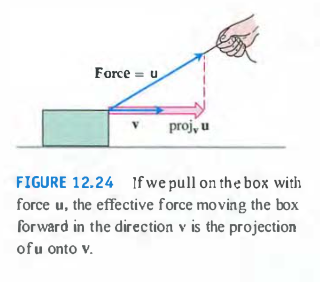
\includegraphics[scale=0.8]{m1_f9}
\end{center}

\bigskip

This motivates the idea of ``projecting" the vector $\bm{u}$ onto the vector $\bm{v}$. The idea is to determine ``how much" of the vector $\bm{u}$ is pointing in the direction of $\bm{v}$. We can look at the drawing above to help us derive a formula for this projection. Our notation for this vector will be $\text{proj}_{\bm{v}} \bm{u}$, which is read ``the vector projection of $\bm{u}$ onto $\bm{v}$".
\begin{align*}
\text{proj}_{\bm{v}} \bm{u} &= \left(||\bm{u}|| \cos(\theta)\right) \frac{\bm{v}}{||\bm{v}||}\\
&= \left(\frac{||\bm{u}|| ||\bm{v}|| \cos(\theta)}{||\bm{v}||} \right) \frac{\bm{v}}{||\bm{v}||}\\
&= \left( \frac{\bm{u}\cdot\bm{v}}{||\bm{v}||} \right) \frac{\bm{v}}{||\bm{v}||}\\
&= \left(\frac{\bm{u}\cdot\bm{v}}{||\bm{v}||^2}\right)\bm{v}.
\end{align*}

\bigskip

\hrulefill

\bigskip

\begin{definition}
The \textbf{vector projection} of $\bm{u}$ onto $\bm{v}$ is the vector
\begin{align*}
\text{proj}_{\bm{v}} \bm{u} = \left(\frac{\bm{u}\cdot\bm{v}}{||\bm{v}||^2}\right)\bm{v}.
\end{align*}
The \textbf{scalar component} of $\bm{u}$ in the direction of $\bm{v}$ is the scalar
\begin{align*}
||\bm{u}||\cos(\theta) = \frac{\bm{u}\cdot\bm{v}}{||\bm{v}||} = \bm{u} \cdot \frac{\bm{v}}{||\bm{v}||}.
\end{align*}
\end{definition}

\bigskip

\textbf{Notes:}
\begin{itemize}
\item If the angle $\theta$ between $\bm{u}$ and $\bm{v}$ is obtuse, our scalar component will be negative.
\item Neither the vector projection or scalar component depend on the length of $\bm{v}$, only its direction.
\end{itemize}

\bigskip

\hrulefill

\bigskip

\begin{example}
Find the vector projection of $\bm{u} = 6\bm{i} +3\bm{j} + 2\bm{k}$ onto $\bm{v} = \bm{i}-2\bm{j} - 2\bm{k}$ and the scalar component of $\bm{u}$ in the direction of $\bm{v}$.\\

\smallskip

\begin{align*}
\text{proj}_{\bm{v}} \bm{u} &= \frac{\bm{u}\cdot\bm{v}}{||\bm{v}||^2} \bm{v}\\
&= \frac{6-6-4}{1+4+4} (\bm{i}-2\bm{j}-2\bm{k})\\
&= -\frac{4}{9} \bm{i} + \frac{8}{9}\bm{j} + \frac{8}{9} \bm{k}.
\end{align*}
The scalar component is
\begin{align*}
\bm{u} \cdot \frac{\bm{v}}{||\bm{v}||} &= (6\bm{i} +3\bm{j} + 2\bm{k}) \cdot \left(\frac{1}{3}\bm{i} - \frac{2}{3}\bm{j}-\frac{2}{3}\bm{k}\right)\\
&= 2-2-\frac{4}{3} = \frac{-4}{3}.
\end{align*}
\end{example}

\bigskip

\hrulefill

\bigskip

\begin{example}
Find the vector projection of a force $\bm{F} = 5\bm{i}+2\bm{j}$ onto $\bm{v} = \bm{i}-3\bm{j}$ and the scalar component of $\bm{F}$ in the direction of $\bm{v}$. (Draw picture).\\

\smallskip

The vector projection is
\begin{align*}
\text{proj}_{\bm{v}} \bm{F} &= \left(\frac{\bm{F}\cdot\bm{v}}{||\bm{v}||^2}\right) \bm{v}\\
&= \frac{5-6}{1+9} (\bm{i}-3\bm{j})\\
&= -\frac{1}{10}\bm{i} + \frac{3}{10}\bm{j}.
\end{align*}
The scalar component of $\bm{F}$ in the direction of $\bm{v}$ is
\begin{align*}
\frac{\bm{F}\cdot\bm{v}}{||\bm{v}||} = \frac{5-6}{\sqrt{1+9}} = -\frac{1}{\sqrt{10}}.
\end{align*}
\end{example}

\newpage

% --------------------------------------------------------------
%                         Sec 12.4
% --------------------------------------------------------------

\section{The Cross Product (12.4)}

We are going to continue to build our understanding of what type of operations we can perform on vectors. The emphasis (especially in this section) should be first understanding conceptually the operations we are performing and then understanding how to actually perform the operations.

\bigskip

There are two types of ``multiplication" that can be performed on vectors. This first (which we have already seen) is the dot product. Roughly speaking, this allowed us to see ``how much" of a vector is pointing in the direction of another vector. The second form of vector multiplication is called the \textbf{cross product}. While this is a form of vector multiplication just like the dot product, it behaves extremely differently. For one, the cross product produces a vector, not a scalar. The cross product allows us to see how a plane is oriented in three-dimensional space. 

\bigskip

\hrulefill

\bigskip

Take two nonzero vectors $\bm{u}$ and $\bm{v}$ in three-dimensions. If these vectors are not parallel, they determine a plane. The cross product takes these two vectors and produces a third vector $\bm{u} \times \bm{v}$ which points in a direction perpendicular to the plane.

\bigskip

\begin{center}
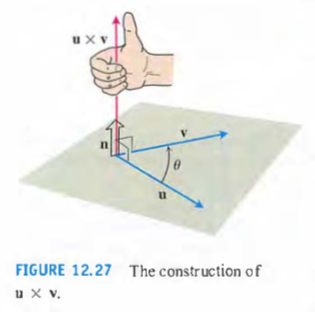
\includegraphics[scale=0.8]{m1_f10}
\end{center}

\bigskip

\begin{definition}
The \textbf{cross product} of two vectors $\bm{u}$ and $\bm{v}$ is
\begin{align*}
\bm{u} \times \bm{v} = (||\bm{u}|| ||\bm{v}|| \sin(\theta)) \bm{n}
\end{align*}
where $\bm{n}$ is the unit (normal) vector perpendicular to the plane formed by $\bm{u}$ and $\bm{v}$.
\end{definition}

\bigskip

We'll see later how to calculate this, but first lets look at a few properties of the cross product.

\bigskip

\hrulefill

\bigskip

The cross product can be used to determine when two vectors are parallel. 

\begin{proposition}
The cross product of two nonzero vectors $\bm{u}$ and $\bm{v}$ is parallel if and only if $\bm{u} \times \bm{v} = \bm{0}$.
\end{proposition}

\bigskip

\textbf{Note:} This is not the only way to determine if two vectors are parallel! In fact, it is usually a very inefficient way to check if two vectors are parallel. A much quicker way would be to simply check if one vector is a scalar multiple of another.

\bigskip

\hrulefill

\bigskip

\begin{definition}{(Properties of the Cross Product)}
Let $\bm{u}$, $\bm{v}$, $\bm{w}$ be any vectors and let $r, s$ be scalars. Then the following are true.
\begin{itemize}
\item $(r\bm{u}) \times (s\bm{v}) = (rs)(\bm{u}\times\bm{v})$
\item $\bm{u} \times (\bm{v}+\bm{w}) = \bm{u} \times \bm{v} + \bm{u} \times \bm{w}$
\item $\bm{v} \times \bm{u} = -(\bm{u} \times \bm{v})$
\item $(\bm{v}+\bm{w}) \times \bm{u} = \bm{v} \times \bm{u} + \bm{w} \times \bm{u}$
\item $\bm{0} \times \bm{u} = \bm{0}$
\item $\bm{u} \times (\bm{v} \times \bm{w}) = (\bm{u} \cdot \bm{w})\bm{v} - (\bm{u}\cdot\bm{v})\bm{w}$
\end{itemize}
\end{definition}

\bigskip

\textbf{Notes}
\begin{itemize}
\item The last property above implies that the cross product is \textit{not} associative. That is, $(\bm{u} \times \bm{v}) \times \bm{w} \neq \bm{u} \times (\bm{v} \times \bm{w})$.
\item The third property above has a nice geometric representation.

\bigskip

\begin{center}
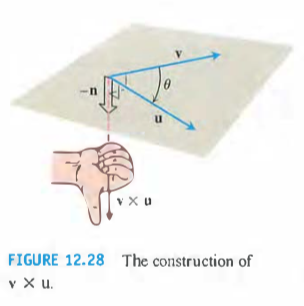
\includegraphics[scale=0.8]{m1_f11}
\end{center}

\end{itemize}

\bigskip

\hrulefill

\bigskip

The cross product can be used to find the area of a parallelogram. 

\bigskip

\begin{center}
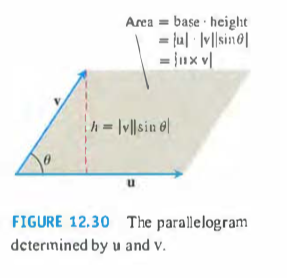
\includegraphics[scale=0.8]{m1_f12}
\end{center}

\bigskip

Note above that we used the following:
\begin{align*}
||\bm{u}\times\bm{v}|| = ||\bm{u}|| ||\bm{v}|| |\sin(\theta)| ||\bm{n}|| = ||\bm{u}|| ||\bm{v}|| \sin(\theta).
\end{align*}

\bigskip

\hrulefill

\bigskip

Using the above properties, we could derive a formula for the cross product of two vectors using only the cartesian coordinate representation of the vectors. That is, we could find
\begin{align*}
\bm{u} \times \bm{v} &= (u_1 \bm{i} + u_2 \bm{j} + u_3 \bm{k}) \times (v_1 \bm{i} + v_2 \bm{j} + v_3 \bm{k})\\
&= (u_2v_3-u_3v_2)\bm{i} - (u_1v_3-u_3v_1)\bm{j}+(u_1v_2-u_2v_1)\bm{k}.
\end{align*}
This is a nightmare to memorize, so we can instead represent this as the determinant of a $2 \times 2$ matrix.

\bigskip

\begin{proposition}
If $\bm{u} = u_1\bm{i} + u_2\bm{j} + u_3\bm{k}$ and $\bm{v} = v_1\bm{i} + v_2\bm{j} + v_3\bm{k}$, then
\begin{align*}
\bm{u} \times \bm{v} = \begin{vmatrix} \bm{i} & \bm{j} & \bm{k} \\ u_1 & u_2 & u_3 \\ v_1 & v_2 & v_3 \end{vmatrix}.
\end{align*}
\end{proposition}

\bigskip

\hrulefill

\bigskip

With this definition, we just need to know how to calculate determinants. The determinant of a $2\times 2$ matrix is
\begin{align*}
\begin{vmatrix} a & b \\ c & d \end{vmatrix} = ad-bc.
\end{align*}
The determinant of a $3\times 3$ matrix is
\begin{align*}
\begin{vmatrix} a_1 & a_2 & a_3 \\ b_1 & b_2 & b_3 \\ c_1 & c_2 & c_3 \end{vmatrix} = a_1 \begin{vmatrix} b_2 & b_3 \\ c_2 & c_3 \end{vmatrix} - a_2 \begin{vmatrix} b_1 & b_3 \\ c_1 & c_3 \end{vmatrix} + a_3 \begin{vmatrix} b_1 & b_2 \\ c_1 & c_2 \end{vmatrix}.
\end{align*}

\bigskip

\hrulefill

\bigskip

\begin{example}
Find $\bm{u} \times \bm{v}$ and $\bm{v} \times \bm{u}$ if $\bm{u} = \langle 2, 1, 1 \rangle$ and $\bm{v} = \langle -4, 3, 1 \rangle$.\\

\smallskip

\begin{align*}
\bm{u} \times \bm{v} &= \begin{vmatrix} \bm{i} & \bm{j} & \bm{k} \\ 2 & 1 & 1 \\ -4 & 3 & 1 \end{vmatrix}\\
&= \begin{vmatrix} 1 & 1 \\ 3 & 1 \end{vmatrix}\bm{i} - \begin{vmatrix} 2 & 1 \\ -4 & 1 \end{vmatrix}\bm{j} + \begin{vmatrix} 2 & 1 \\ -4 & 3 \end{vmatrix}\bm{k}\\
&= -2\bm{i} - 6\bm{j} + 10\bm{k}\\
\bm{v} \times \bm{u} &= -(\bm{u} \times \bm{v}) = 2\bm{i} + 6\bm{j} -10\bm{k}.
\end{align*}
\end{example}

\bigskip

\hrulefill

\bigskip

\begin{example}
Find a vector perpendicular to the plane of $P(1,-1,0), Q(2,1,-1), R(-1,1,2)$.\\

\bigskip

\begin{center}
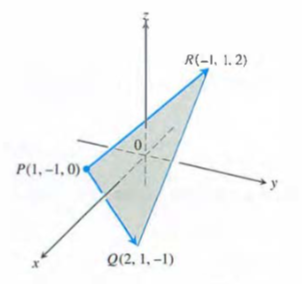
\includegraphics[scale=0.7]{m1_f13}
\end{center}

\bigskip

We are looking for the vector $\vec{PQ} \times \vec{PR}$. So note that
\begin{align*}
\vec{PQ} &= \langle 2-1, 1+1, -1-0 \rangle = \langle 1,2,-1 \rangle\\
\vec{PR} & = \langle -1-1, 1+1, 2-0 \rangle = \langle -2, 2, 2 \rangle\\
\vec{PQ} \times \vec{PR} &= \begin{vmatrix} \bm{i} & \bm{j} & \bm{k} \\ 1 & 2 & -1 \\ -2 & 2 & 2 \end{vmatrix}\\
&= \begin{vmatrix} 2 & -1 \\ 2 & 2 \end{vmatrix} \bm{i} - \begin{vmatrix} 1 & -1 \\ -2 & 2 \end{vmatrix} \bm{j} + \begin{vmatrix} 1 & 2 \\ -2 & 2 \end{vmatrix} \bm{k}\\
&= 6\bm{i} + 6\bm{k}.
\end{align*}
\end{example}

\bigskip

\hrulefill

\bigskip

\begin{example}
Find the area of the triangle with vertices $P(1,-1,0), Q(2,1,-1), R(-1,1,2)$.\\

\smallskip

The area of the triangle is half of the area of the parallelogram defined by the vectors $\vec{PQ}$ and $\vec{PR}$. So we have
\begin{align*}
A &= \frac{1}{2} ||\vec{PQ} \times \vec{PR}||\\
&=\frac{1}{2} ||6\bm{i}+6\bm{k}||\\
&= \frac{1}{2} \sqrt{6^2+6^2}\\
&=\frac{1}{2} 6\sqrt{2}\\
&= 3\sqrt{2}.
\end{align*}
\end{example}

\bigskip

\hrulefill

\bigskip

\begin{example}
Find a unit vector perpendicular to the plane of $P(1,-1,0), Q(2,1,-1), R(-1,1,2)$.\\

\smallskip

We already found a vector perpendicular to the plane in the example above. So we simply need to make that vector a unit vector.
\begin{align*}
\bm{n} &= \frac{\vec{PQ} \times \vec{PR}}{||\vec{PQ} \times \vec{PR}||}\\
&= \frac{6\bm{i} + 6\bm{k}}{6\sqrt{2}}\\
&= \frac{1}{\sqrt{2}} \bm{i} + \frac{1}{\sqrt{2}} \bm{k}.
\end{align*}
\end{example}

\bigskip

\hrulefill

\bigskip

\begin{definition}
The \textbf{triple scalar product} or \textbf{box product} of the vectors $\bm{u},\bm{v}$ and $\bm{w}$ (in that order) is $(\bm{u} \times \bm{v}) \cdot \bm{w}$.
\end{definition}

\bigskip

The box product can be used to find the height volume of a parellelepiped. How?

\bigskip

\begin{center}
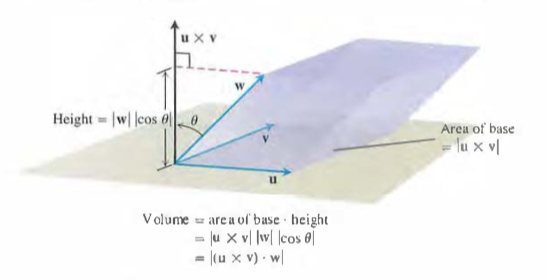
\includegraphics[scale=0.8]{m1_f14}
\end{center}

\bigskip

\begin{proposition}
$(\bm{u} \times \bm{v}) \cdot \bm{w} = \begin{vmatrix} u_1 & u_2 & u_3 \\ v_1 & v_2 & v_3 \\ w_1 & w_2 & w_3 \end{vmatrix}$
\end{proposition}

\bigskip

\hrulefill

\bigskip

\begin{example}
Find the volume of the parallelepiped determined by $\bm{u} = \langle 1, 2, -1 \rangle$, $\bm{v} = \langle -2, 0, 3 \rangle$ and $\bm{w} = \langle 0, 7, -4 \rangle$.\\

\smallskip

\begin{align*}
(\bm{u} \times \bm{v}) \cdot \bm{w} &= \begin{vmatrix} 1 & 2 & -1 \\ -2 & 0 & 3 \\ 0 & 7 & -4 \end{vmatrix}\\
&= -23.
\end{align*}
Therefore the volume of the box is $V = |(\bm{u} \times \bm{v}) \cdot \bm{w}| = 23$.
\end{example}

\newpage

% --------------------------------------------------------------
%                         Sec 12.5
% --------------------------------------------------------------

\section{Lines and Planes in Space (12.5)}

We know all about lines in two-dimensions. The nice thing about this section is that most of our knowledge of lines in two-dimensions will transfer over nicely to lines in three dimensions. In two-dimensions we can define a line either by specifying two points in the plane or by giving a point and the slope of the line. In three-dimensions we can also specify a line by giving two points in space or we can define a line by giving a point on the line and a vector that you can think of as specifying the slope of the line. Consider the following drawing.

\bigskip

\begin{center}
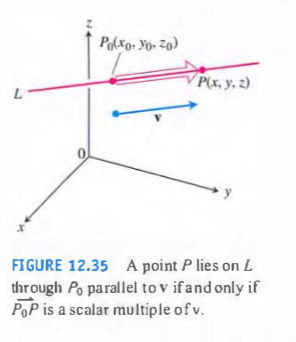
\includegraphics[scale=0.7]{m1_f17}
\end{center}

\bigskip

The line is defined as all points $P(x,y,z)$ for which $\vec{P_0P}$ is parallel to $\bm{v}$. We can write this as the line is defined as all points $P$ satisfying $\vec{P_0P} = tv$ for some parameter $t$. Expanding this gives
\begin{align*}
(x-x_0)\bm{i}+(y-y_0)\bm{j}+(z-z_0)\bm{k} = t(v_1\bm{i}+v_2\bm{j}+v_3\bm{k})
\end{align*}
or
\begin{align*}
x\bm{i}+y\bm{j}+z\bm{k} = x_0\bm{i} + y_0\bm{j}+z_0\bm{k}+ t(v_1\bm{i}+v_2\bm{j}+v_3\bm{k}).
\end{align*}
This leads to the following definition.

\begin{definition}
A \textbf{vector equation} for the line $L$ through $P_0(x_0,y_0,z_0)$ parallel to $\bm{v}$ is
\begin{align*}
\bm{r}(t) = \bm{r}_0+t\bm{v}, \ \ \ -\infty < t < \infty
\end{align*}
where $\bm{r}$ is the position vector of a point $P(x,y,z)$ on $L$ and $\bm{r}_0$ is the position vector of $P_0(x_0,y_0,z_0)$.
\end{definition}

\bigskip

We could also write this component wise.

\begin{definition}
The \textbf{standard parametrization} of the line through $P_0(x_0,y_0,z_0)$ parallel to $\bm{v} = v_1 \bm{i} + v_2\bm{j} + v_3\bm{k}$ is
\begin{align*}
x=x_0+tv_1 \ \ \ y=y_0+tv_2, \ \ \ z=z_0+tv_3 \ \ \ -\infty<t<\infty.
\end{align*}
\end{definition}

\bigskip

\hrulefill

\bigskip

\begin{example}
Find a vector equation and parametric equations for the line through $P(-3,2,-3)$ and $Q(1,-1,4)$.\\

\smallskip

We can use $P$ as our point on the line, so we now just need a vector parallel to the line. We can find this by noting that $\vec{PQ}$ is parallel to the line. So we have
\begin{align*}
\vec{PQ} &= \langle 1-(-3), -1-2, 4-(-3) \rangle\\
&= \langle 4, -3, 7 \rangle.
\end{align*}
So our vector equation is
\begin{align*}
\bm{r}(t) &= \langle -3, 2, -3 \rangle + t \langle 4, -3, 7 \rangle\\
&= \langle -3+4t, 2-3t, -3+7t \rangle.
\end{align*}
The above work also gives our parametric equations:
\begin{align*}
x= -3+4t \ \ \ y=2-3t \ \ \ -3+7t.
\end{align*}
Since parametric equations aren't unique, there is more than one way to write the above equations.
\end{example}

\bigskip

\hrulefill

\bigskip

\begin{example}
Parametrize the line segment joining the points $P(-3,2,-3)$ and $Q(1,-1,4)$.\\

\bigskip

\begin{center}
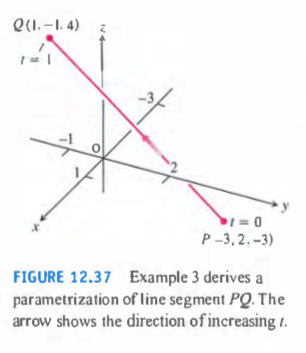
\includegraphics[scale=0.7]{m1_f15}
\end{center}

\bigskip

We found the line passing through $P$ and $Q$ in the previous example, so all we need to do is adjust the interval of our parameter to make the point start at $P$ and end at $Q$. Note that if $t=0$ in our parametric equations then we have the point $P(-3,2,-3)$ and if $t=1$ we have $Q(1,-1,4)$. Thus our parametrization for the line segment is
\begin{align*}
x= -3+4t \ \ \ y=2-3t \ \ \ z=-3+7t \ \ \ 0 \leq t \leq 1.
\end{align*}
\end{example}

\bigskip

\hrulefill

\bigskip

Suppose we want to find the distance in space from a point $S$ to a line that passes through a point $P$ parallel to a vector $\bm{v}$.

\bigskip

\begin{center}
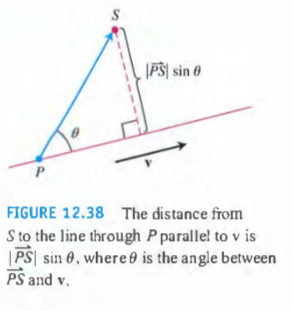
\includegraphics[scale=0.7]{m1_f18}
\end{center}

\bigskip

The previous drawing leads us to the following.

\begin{proposition}
The distance from a point $S$ to a line through $P$ and parallel to $\bm{v}$ is
\begin{align*}
d = ||\vec{PS}||\sin(\theta) = \frac{||\vec{PS}\times\bm{v}||}{||\bm{v}||}.
\end{align*}
\end{proposition}

\bigskip

\hrulefill

\bigskip

\begin{example}
Find the distance from the point $S(1,1,5)$ to the line given by the parametric equations
\begin{align*}
x=1+t \ \ \ y=3-t \ \ \ z=2t.
\end{align*}
We need to express this line in terms of a point $P$ on the line and a vector parallel to the line. To find the point $P$ we can set $t=0$ to get $P(1,3,0)$. To find the vector parallel to the line we just need to take the coefficients on the $t$ terms to get $\bm{v} = \langle 1, -1, 2 \rangle$. So now we have
\begin{align*}
\vec{PS} &= \langle 1-1, 1-3, 5-0 \rangle\\
&= \langle 0, -2, 5 \rangle.
\end{align*}
To find our distance $d$ we need to compute $\vec{PS} \times \bm{v}$, so we see
\begin{align*}
\vec{PS} \times \bm{v} &= \begin{vmatrix} \bm{i} & \bm{j} & \bm{k} \\ 0 & -2 & 5 \\ 1 & -1 & 2 \end{vmatrix}\\
&= \bm{i} + 5\bm{j} + 2\bm{k}.
\end{align*}
Thus we have
\begin{align*}
d &= \frac{||\vec{PS} \times \bm{v}||}{||\bm{v}||}\\
&= \frac{\sqrt{1+25+4}}{\sqrt{1+1+4}}\\
&= \sqrt{5}.
\end{align*}
\end{example}

\bigskip

\hrulefill

\bigskip

A plane in space is completely determined from a point in the plane and the ``tilt" or orientation of the plane in space. We encode the information of a planes orientation by specifying a vector perpendicular, or normal, to the plane.

\bigskip

\begin{center}
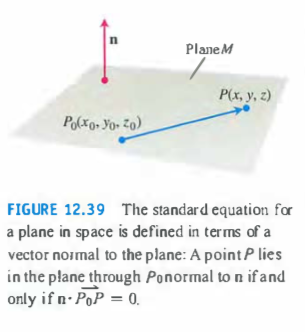
\includegraphics[scale=0.7]{m1_f19}
\end{center}

\bigskip

The plane $M$ in the above figure is the set of all points $P(x,y,z)$ for which $\vec{P_0P}$ is orthogonal to $\bm{n}$. That is to say, the plane $M$ is the set of all points $P$ such that $\bm{n} \cdot \vec{P_0P} = 0$. This leads to the following.

\bigskip

\begin{definition}
The plane through $P_0(x_0,y_0,z_0)$ normal to $\bm{n} = A\bm{i}+B\bm{j}+C\bm{k}$ has
\begin{align*}
\text{Vector equation:} \ \ \ \ \ &\bm{n}\cdot\vec{P_0P} = 0\\
\text{Component equation:} \ \ \ &A(x-x_0)+B(y-y_0)+C(z-z_0)=0\\
\text{Component equation simplified:} \ \ \ &Ax+By+Cz=D \ \ \text{where}\\ 
&D=Ax_0+By_0+Cz_0.
\end{align*}
\end{definition}

\bigskip

\hrulefill

\bigskip

\begin{example}
Find an equation for the plane through $P_0(-3,0,7)$ perpendicular to $\bm{n} = \langle 5,2,-1 \rangle$.

\smallskip

For this example it is probably easiest to find the equation for the plane in component form, so we have
\begin{align*}
5(x-(-3)) + 2(y-0)+(-1)(z-7) &= 0\\
\Rightarrow 5x+15+2y-z+7 &=0\\
\Rightarrow 5x+2y-z&=-22.
\end{align*}
\end{example}

\bigskip

\hrulefill

\bigskip

\begin{example}
Find an equation for the plane through $A(0,0,1)$, $B(2,0,0)$, and $C(0,3,0)$.

\smallskip

We need to find a vector normal to this plane and then we can use any one of the given points as our point used to define the plane. To find a vector normal to this plane we could find a vector perpendicular to both of the vectors $\vec{AB}$ and $\vec{AC}$. This means finding a cross product.
\begin{align*}
\vec{AB} \times \vec{AC} &= \begin{vmatrix} \bm{i} & \bm{j} & \bm{k} \\ 2 & 0 & -1 \\ 0 & 3 & -1 \end{vmatrix}\\
&= 3 \bm{i} + 2\bm{j} + 6\bm{k}.
\end{align*}
So now the equation of our plane (arbitrarily using the point $A$) is
\begin{align*}
3(x-0)+2(y-0)+6(z-1) &= 0\\
\Rightarrow 3x+2y+6z &=6.
\end{align*}
\end{example}

\bigskip

\hrulefill

\bigskip

In two dimensions we know that two lines are parallel if and only if they have the same direction. We can extend this intuition to three dimensions where we know that two planes are parallel if and only if their normal vectors are parallel ($\bm{n}_1=k \bm{n}_2$). Two planes that are not parallel intersect in a line.

\bigskip

\hrulefill

\bigskip

\begin{example}
Find parametric equations for the line in which the planes $3x-6y-2z=15$ and $2x+y-2z=5$ intersect.

\smallskip

We need to find a vector parallel to the line and a point on the line. The easiest way to find a point where the two planes intersect is to set one of the coordinates to zero and solve for the other two coordinates. So we'll arbitrarily set $z=0$ to get
\begin{align*}
3x-6y = 15 \ \ \ 2x+y=5
\end{align*}
which gives the point $(3,-1,0)$ as one point at which the planes intersect. To find the vector which points in the direction of the line, note that the line of intersection of two planes is perpendicular to both planes' normal vectors.

\bigskip

\begin{center}
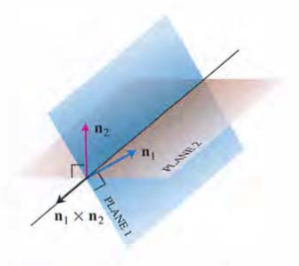
\includegraphics[scale=0.7]{m1_f16}
\end{center}

\bigskip
So we need to find $\bm{n}_1 \times \bm{n_2}$.
\begin{align*}
\bm{n}_1 \times \bm{n_2} &= \begin{vmatrix} \bm{i} & \bm{j} & \bm{k} \\ 3 & -6 & -2 \\ 2 & 1 & -2 \end{vmatrix}\\
&= 14\bm{i} + 2\bm{j} + 15\bm{k}.
\end{align*}
Therefore the parametric equations for the line we seek are
\begin{align*}
x=3+14t \ \ \ y=-1+2t \ \ \ z=15t.
\end{align*}
\end{example}

\bigskip

\hrulefill

\bigskip

If $P$ is a point on a plane with normal $\bm{n}$, the distance from any point $S$ in space to the plane is the length of the vector projection of $\bm{PS}$ onto $\bm{n}$. That is
\begin{align*}
d = \left| \vec{PS} \cdot \frac{\bm{n}}{||\bm{n}||} \right|.
\end{align*}
(Draw the next picture without specific coordinates.)

\bigskip

\begin{center}
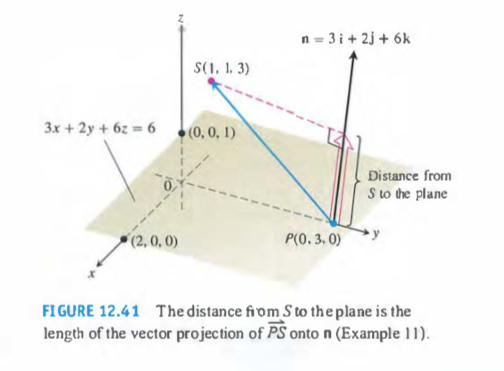
\includegraphics[scale=0.7]{m1_f20}
\end{center}

\bigskip

\hrulefill

\bigskip

\begin{example}
Find the distance from $S(1,1,3)$ to the plane $3x+2y+6z=6$.

\smallskip

We need to find a point $P$ in the plane and project $\vec{PS}$ onto some vector $\bm{n}$ which is normal to the plane. To find the point $P$ we'll choose to find one of the intercepts of the plane. So arbitrarily set $x=0$ and $z=0$ to get the point $(0,3,0)$. Our normal vector we can read off from the equation of the plane as $\bm{n} = \langle 3, 2, 6 \rangle$. So now we have
\begin{align*}
\vec{PS} &= \langle 1-0, 1-3, 3-0 \rangle\\
&= \langle 1, -2, 3 \rangle.
\end{align*}
Which means our distance is
\begin{align*}
d &= \left| \vec{PS} \cdot \frac{\bm{n}}{||\bm{n}||} \right|\\
&= \left| \langle 1, -2, 3 \rangle \cdot \bigg\langle \frac{3}{7}, \frac{2}{7}, \frac{6}{7} \bigg\rangle \right|\\
&= \frac{17}{7}.
\end{align*}
\end{example}

\bigskip

\hrulefill

\bigskip

The angle between two planes is defined to be the acute angle between their normal vectors.

\bigskip

\begin{center}
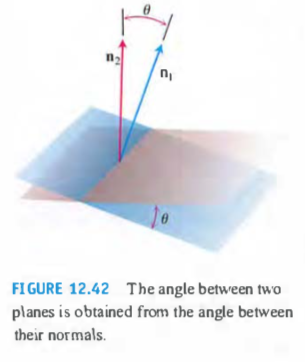
\includegraphics[scale=0.7]{m1_f21}
\end{center}

\bigskip

\hrulefill

\bigskip

\begin{example}
Find the angle between the planes $3x-6y-2z=15$ and $2x+y-2z=5$.

\smallskip

The normal vectors here are $\bm{n}_1 = \langle 3, -6, -2 \rangle$ and $\bm{n}_2 = \langle 2, 1, -2 \rangle$. The angle between these vectors is
\begin{align*}
\theta &= \arccos\left(\frac{\bm{n}_1 \cdot \bm{n}_2}{||\bm{n}_1|| ||\bm{n}_2||}\right)\\
&= \arccos \left(\frac{4}{21}\right).
\end{align*}
\end{example}

\newpage

% --------------------------------------------------------------
%                         Sec 12.6
% --------------------------------------------------------------

\section{Cylinders and Quadric Surfaces (12.6)}

At this point we know only how to plot lines, planes and spheres in three dimensions. We will add to this list and emphasize visualization and understanding as opposed to memorization.

\bigskip

\begin{definition}
A \textbf{cylinder} is a surface that is generated by moving a straight line along a given planar curve while holding the line parallel to a given fixed line. The curve is called a \textbf{generating curve} for the cylinder.
\end{definition}

\bigskip

\begin{center}
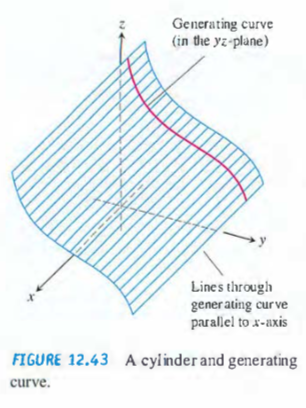
\includegraphics[scale=0.7]{m1_f22}
\end{center}

\bigskip

\textbf{Notes:}
\begin{itemize}
\item This is more general than what most people think of as a cylinder! However, we can recover the geometric notion of a cylinder we already have by letting the generating curve be a circle, say $x^2+y^2=1$ and letting the lines of the cylinder be parallel to $z=0$.
\item The key feature of cylinders is that their equations contain exactly two of the three variables.
\end{itemize}

\bigskip

\hrulefill

\bigskip

\begin{example}
Find an equation for the cylinder made by the lines parallel to the $z$-axis that pass through the parabola $y=x^2, z=0$.\\

\bigskip

\begin{center}
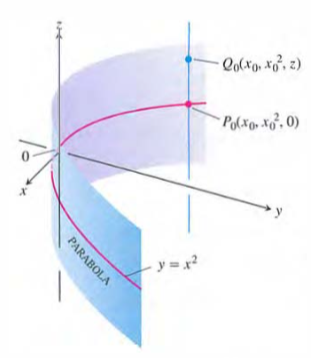
\includegraphics[scale=0.6]{m1_f23}
\end{center}

\bigskip

The cylinder described is the parabola $y=x^2$ in the $xy$-plane and any point on the $z$-axis. So we call this ``the cylinder $y=x^2$". We could write the equation for this cylinder as $y-x^2=0$.
\end{example}

\bigskip

\hrulefill

\bigskip

This last example leads to a general rule. Any curve $f(x,y) = c$ defines a cylinder parallel to the $z$-axis whose equation is also $f(x,y) = c$. Any curve $g(x,z) = c$ defines a cylinder parallel to the $y$-axis whose equation is also $g(x,z) = c$. Any curve $h(y,z) = c$ defines a cylinder parallel to the $x$-axis whose equation is also $h(y,z) = c$. This is useful, but keep in mind that the axis of a cylinder does not need to be parallel to a coordinate axis.

\bigskip

\hrulefill

\bigskip

At this point we will briefly review the concept of \textit{conic sections}. Conic sections are the cures given by parabolas, ellipses, and hyperbolas. (Draw pictures of each of the following.)
\begin{itemize}
\item A parabola is given in standard form by $y=\frac{x^2}{4p}$.
\item An ellipse is given by the equation $\frac{x^2}{a^2}+\frac{y^2}{b^2} = 1$.
\item A hyperbola is given by the equation $\frac{x^2}{a^2}-\frac{y^2}{b^2} = 1$.
\end{itemize}

\bigskip

\hrulefill

\bigskip

\begin{definition}
A \textbf{quadric surface} is the graph in space of a second-degree equation in $x$, $y,$ and $z$.
\end{definition}

\bigskip

There are six basic types of of quadric surfaces:
\begin{itemize}
\item An ellipsoid is given by $\frac{x^2}{a^2} + \frac{y^2}{b^2} + \frac{z^2}{c^2} = 1$.
\item An elliptical paraboloid is given by $\frac{x^2}{a^2} + \frac{y^2}{b^2} = \frac{z}{c}$.
\item An elliptical cone is given by $\frac{x^2}{a^2} + \frac{y^2}{b^2} = \frac{z^2}{c^2}$.
\item A hyperboloid of one sheet is given by $\frac{x^2}{a^2} + \frac{y^2}{b^2} - \frac{z^2}{c^2} = 1$.
\item A hyperboloid of two sheets is given by $\frac{z^2}{c^2} - \frac{x^2}{a^2} - \frac{y^2}{b^2} = 1$.
\item A hyperbolic paraboloid is given by $\frac{y^2}{b^2} - \frac{x^2}{a^2} = \frac{z}{c}, \ c>0$.
\end{itemize}

\bigskip

I would encourage you \textbf{not} to memorize these. Instead you should think about (and this is how these surfaces get their names) the cross sections of these surfaces when cut by one of the principle axes. For instance, if we cut an ellipsoid by any of the axes $x=0$, $y=0$, $z=0$ we get an ellipse in two dimensions. Think about doing this for the other shapes.

\bigskip

\hrulefill

\bigskip

\begin{example}
Sketch the ellipsoid
\begin{align*}
\frac{x^2}{a^2} + \frac{y^2}{b^2} + \frac{z^2}{c^2} = 1.
\end{align*}

\bigskip

\begin{center}
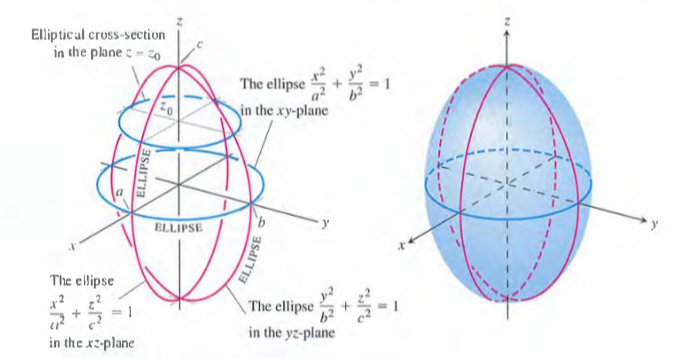
\includegraphics[scale=0.7]{m1_f24}
\end{center}
\end{example}

\bigskip

\hrulefill

\bigskip

\begin{example}
Sketch the hyperbolic paraboloid
\begin{align*}
\frac{y^2}{b^2} - \frac{x^2}{a^2} = \frac{z}{c}.
\end{align*}

\bigskip

\begin{center}
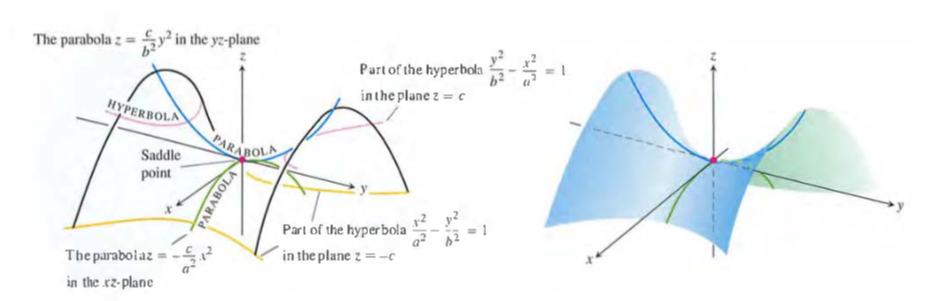
\includegraphics[scale=0.55]{m1_f25}
\end{center}
\end{example}

\newpage

% --------------------------------------------------------------
%                         Sec 13.1
% --------------------------------------------------------------

\section{Curves in Space and Their Tangents (13.1)}

Now that we understand points and vectors in space, lets look at how certain functions behave in space.

\bigskip

\begin{definition}
A \textbf{vector function} or \textbf{vector valued function} parametrized by $t\in I$ is given by
\begin{align*}
\bm{r}(t) = f(t) \bm{i} + g(t)\bm{j} + h(t)\bm{k} = \langle f(t), g(t), h(t) \rangle, \ t\in I.
\end{align*}
We call $f,g,h$ the \textbf{component functions} and call the collection of points $(x,y,z) = (f(t),g(t),h(t)), \ t\in I$ a \textbf{curve} in space.
\end{definition}

\bigskip

\textbf{Notes:}
\begin{itemize}
\item The function $\bm{r}$ defined above is a function from $\bm{R}$ to $\bm{R}^3$. This is different than functions we have seen before, but it turns out these behave very similarly to functions from $\bm{R}$ to $\bm{R}$.
\item We often will think of $\bm{r}(t)$ as the position of a particle in space at any time $t$.
\end{itemize}

\bigskip

\hrulefill

\bigskip

\begin{example}
Plot (or describe) the following vector valued functions.\\
\begin{itemize}
\item[1.] $\bm{r}(t) = \langle \cos(t), \sin(t), t \rangle$

\bigskip

\begin{center}
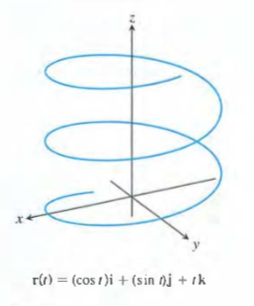
\includegraphics[scale=0.7]{m1_f26}
\end{center}

\bigskip

\item[2.] $\bm{r}(t) = t\bm{i} + t^2\bm{j} + \bm{k}$

\bigskip

This is a parabola in th $xy$-plane that is shifted up one on the $z$-axis (draw sketch).

\bigskip

\item[3.] $\bm{r}(t) = \langle 1+t, 3-4t, -2+5t \rangle$

\bigskip

This is the line passing through the point $(1,3,-2)$ parallel to the vector $\langle 1, -4, 5 \rangle$.

\bigskip

\begin{center}
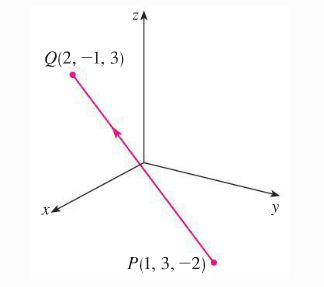
\includegraphics[scale=0.7]{m1_f27}
\end{center}

\bigskip

\end{itemize}
\end{example}

\bigskip

\hrulefill

\bigskip

It turns out that limits, continuity, and derivatives of vector valued functions are defined almost identically to functions defined over $\bm{R}$.

\bigskip

\begin{definition}
Let $\bm{r}(t) = f(t) \bm{i} + g(t) \bm{j} + h(t) \bm{k}$ be a vector function with domain $D$ and $L$ a vector. We say that $\bm{r}$ has \textbf{limit} $L$ as $t$ approaches $t_0$ and write
\begin{align*}
\lim_{t\to t_0} \bm{r}(t) = \bm{L}
\end{align*}
if, for every number $\epsilon >0$ there exists a corresponding number $\delta >0$ such that for all $t\in D$
\begin{align*}
||\bm{r}(t) - \bm{L}|| < \epsilon \ \ \text{whenever} \ \ 0<|t-t_0|<\delta.
\end{align*}
\end{definition}

\bigskip

If $\bm{L} = \langle L_1, L_2, L_3 \rangle$ then $\lim_{t\to t_0} \bm{r}(t) = \bm{L}$ when
\begin{align*}
\lim_{t\to t_0} f(t) = L_1, \ \ \lim_{t\to t_0} g(t) = L_2 \ \ \lim_{t\to t_0} h(t) = L_3.
\end{align*}
So in practice, we just need to find the limits of the components of $\bm{r}(t)$.

\bigskip

\hrulefill

\bigskip

\begin{example}
Find the indicated limits of the following functions.\\
\begin{itemize}
\item[1.] $\lim_{t \to \pi/4} \bm{r}(t)$ where $\bm{r}(t) = (\cos(t))\bm{i}+(\sin(t))\bm{j} + t\bm{k}$.
\begin{align*}
\lim_{t \to \pi/4} \bm{r}(t) &= \left(\lim_{t \to \pi/4} \cos(t)\right) \bm{i} + \left(\lim_{t \to \pi/4} \sin(t)\right)\bm{j} + \left(\lim_{t \to \pi/4} t\right)\bm{k}\\
&= \frac{\sqrt{2}}{2} \bm{i} + \frac{\sqrt{2}}{2} \bm{j} + \frac{\pi}{2} \bm{k}.
\end{align*}
\item[2.] $\lim_{t \to 1} \bm{r}(t)$ where $\bm{r}(t) = t \bm{i}+t^2\bm{j} + \frac{1}{t} \bm{k}$.
\begin{align*}
\lim_{t \to 1} \bm{r}(t) &= \left(\lim_{t \to 1} t \right) \bm{i} + \left(\lim_{t \to 1} t^2 \right)\bm{j} + \left(\lim_{t \to 1} \frac{1}{t}\right)\bm{k}\\
&= \bm{i} + \bm{j} + \bm{k}.
\end{align*}
\item[3.] $\lim_{t \to 0} \bm{r}(t)$ where $\bm{r}(t) = t \bm{i}+t^2\bm{j} + \frac{1}{t} \bm{k}$.
\begin{align*}
\lim_{t \to 0} \bm{r}(t) &= \left(\lim_{t \to 0} t \right) \bm{i} + \left(\lim_{t \to 0} t^2 \right)\bm{j} + \left(\lim_{t \to 0} \frac{1}{t}\right)\bm{k}.
\end{align*}
The above limit does not exist because $\lim_{t\to 0} \frac{1}{t}$ does not exist.
\end{itemize}
\end{example}

\bigskip

\hrulefill

\bigskip

\begin{definition}
A vector function $\bm{r}(t)$ is \textbf{continuous at a point} $t=t_0$ in its domain if $\lim_{t\to t_0} \bm{r}(t) = \bm{r}(t_0)$. The function is \textbf{continuous} if it is continuous at every point in its domain.
\end{definition}

\bigskip

Similar to our definition of a limit, a vector valued function is continuous at $t=t_0$ if and only if each component of the vector valued function is continuous at $t=t_0$.

\bigskip

\hrulefill

\bigskip

\begin{definition}
The vector function $\bm{r}(t) = f(t) \bm{i} + g(t) \bm{j} + h(t) \bm{k}$ has a \textbf{derivative} (\textbf{is differentiable}) \textbf{at} $t$ if $f, g$, and $h$ have derivatives at $t$. The derivative is the vector function
\begin{align*}
\bm{r}'(t) = \frac{d\bm{r}}{dt} = \lim_{\Delta t \to 0} \frac{\bm{r}(t+\Delta t) - \bm{r}(t)}{\Delta t} = \frac{df}{dt} \bm{i} + \frac{dg}{dt} \bm{j} + \frac{dh}{dt} \bm{k}.
\end{align*}
\end{definition}

\bigskip

If a vector valued function $\bm{r}$ is differentiable at every point of its domain we call it \textbf{differentiable}. Further, we say that the curve traced by $\bm{r}$ is \textbf{smooth} if $\frac{d\bm{r}}{dt}$ is continuous and never $\bm{0}$. A \textbf{piecewise smooth} curve is made up of a finite number of smooth curves pieced together in a continuous fashion. (Draw example of smooth and piecewise smooth curves).

\bigskip

\hrulefill

\bigskip

All of our old rules for computing still apply for vector valued functions (linearity, chain rule, product rule) but we have to be a bit careful when considering the product rule. For the dot product rule we have
\begin{align*}
\frac{d}{dt}\left(\bm{u}(t) \cdot \bm{v}(t)\right) = \bm{u}'(t) \cdot \bm{v}(t) + \bm{u}(t) \cdot \bm{v}'(t),
\end{align*} 
where the order doesn't matter. But for the cross product rule we have
\begin{align*}
\frac{d}{dt}\left(\bm{u}(t) \times \bm{v}(t)\right) = \bm{u}'(t) \times \bm{v}(t) + \bm{u}(t) \times \bm{v}'(t),
\end{align*} 
and the order here most definitely matters.

\bigskip

\hrulefill

\bigskip

If we consider $\bm{r}(t)$ to be the position of a particle, then the vector function $\bm{v}(t) = \bm{r}'(t)$ is the velocity vector, which is tangent to the curve $\bm{r}(t)$ at any point $t=t_0$. The magnitude of $\bm{v}(t)$ is the speed of the particle, and the vector function $\bm{a}(t) = \bm{v}'(t) = \bm{r}''(t)$ is the acceleration of the particle.

\bigskip

\hrulefill

\bigskip

\begin{example}
\begin{itemize}
\item[1.] Find the derivative of the vector valued function $\bm{r}(t) = \langle \cos(t), \sin(t), t \rangle$. What is $\bm{r}'(\pi/2)$?\\
\begin{align*}
\bm{r}'(t) &= \langle -\sin(t), \cos(t), 1 \rangle\\
\bm{r}'(\pi/2) &= \langle -1, 0, 1 \rangle.
\end{align*}
\item[2.] Let the position of a particle be given by $\bm{r}(t) = \langle t^2, \cos(t),\ln(t) \rangle, \ 0<t<\infty$. Find the velocity, speed, and acceleration of this particle.\\
\begin{align*}
\bm{v}(t) &= \bm{r}'(t) = \langle 2t, -\sin(t), \frac{1}{t} \rangle, \ 0<t<\infty\\
s(t) &= ||\bm{v}(t)|| = \sqrt{(2t)^2+(-\sin(t))^2+(\frac{1}{t})^2} = \sqrt{4t^2+\sin^2(t)+\frac{1}{t^2}}\\
\bm{a}(t) &= \bm{v}(t) = \bm{r}''(t) = \langle 2, -\cos(t), -\frac{1}{t^2} \rangle, \ 0<t<\infty.
\end{align*}
\end{itemize}
\end{example}

\newpage

% --------------------------------------------------------------
%                         Sec 13.2
% --------------------------------------------------------------

\section{Integrals of Vector Functions (13.2)}

Because limits of vector valued functions are done component-wise, integrals of vector valued functions can also be handled component-wise.

\bigskip

\begin{definition}
The \textbf{indefinite integral} of $\bm{r}$ with respect to $t$ is the set of all antiderivatives of $\bm{r}$, denoted by $\int \bm{r}(t)dt$. If $\bm{R}$ is any antiderivative of $\bm{r}$, then
\begin{align*}
\int \bm{r}(t)dt = \bm{R}(t) + \bm{C}
\end{align*}
where $\bm{C}$ is  a constant vector.
\end{definition}

\bigskip

\hrulefill

\bigskip

\begin{example}
Integrate the vector valued function $\bm{r}(t) = \cos(t) \bm{i} + \bm{j} - 2t \bm{k}$.\\
We integrate each of the components to get
\begin{align*}
\int \bm{r}(t) dt &= \int (\cos(t) \bm{i} + \bm{j} - 2t \bm{k})dt\\
&= \left(\int \cos(t)dt\right)\bm{i} + \left(\int dt \right) \bm{j} - \left(\int 2tdt \right) \bm{k}\\
&= (\sin(t)+C_1)\bm{i} + (t+C_2) \bm{j} - (t^2+C_2)\bm{k}\\
&= \sin(t) \bm{i} + t\bm{j} - t^2 \bm{k} + \bm{C}.
\end{align*}
\end{example}

\bigskip

\hrulefill

\bigskip

\begin{definition}
If the components of $\bm{r}(t) = f(t) \bm{i} + g(t) \bm{j} + h(t) \bm{k}$ are integrable over $[a,b]$, then so is $\bm{r}$, and the \textbf{definite integral} of $\bm{r}$ from $a$ to $b$ is
\begin{align*}
\int_a^b \bm{r}(t)dt = \left(\int_a^b f(t)dt \right) \bm{i} + \left(\int_a^b g(t)dt \right) \bm{j} + \left(\int_a^b h(t)dt \right) \bm{k}.
\end{align*}
\end{definition}

\bigskip

\hrulefill

\bigskip

\begin{example}
Calculate the definite integral $\int_0^\pi \left(\cos(t) \bm{i} + \bm{j} - 2t \bm{k}\right)dt$.\\
We did the indefinite integral in the last example, so we have
\begin{align*}
\int_0^\pi (\cos(t) \bm{i} + \bm{j} - 2t \bm{k})dt &= \sin(t)\rvert_0^\pi \bm{i} + t\rvert_0^\pi \bm{j} - t^2\rvert_0^\pi \bm{k}\\
&= (0-0)\bm{i} + (\pi-0)\bm{j}-(\pi^2-0^2)\bm{k}\\
&= \pi \bm{j} -\pi^2\bm{k}.
\end{align*}
\end{example}

\newpage

% --------------------------------------------------------------
%                         Sec 13.3
% --------------------------------------------------------------

\section{Arc Length in Space (13.3)}

In Calc II we say the the arc length of a parametrized curve from $t=a$ to $t=b$ is given by $L =  \int_a^b \sqrt{(dx/dt)^2+(dy/dt)^2}dt$. Our formula for length of a curve defined by a vector function then shouldn't be too surprising.

\bigskip

\begin{definition}
The \textbf{length} of a smooth curve $\bm{r}(t) = x(t)\bm{i}+y(t)\bm{j}+z(t)\bm{k}$, $a\leq t\leq b$, that is traced exactly once as $t$ increases from $t=a$ to $t=b$, is
\begin{align*}
L = \int_a^b \sqrt{\left(\frac{dx}{dt}\right)^2+\left(\frac{dy}{dt}\right)^2+\left(\frac{dz}{dt}\right)^2} dt.
\end{align*}
\end{definition}

\bigskip

This definition is the same as
\begin{align*}
L = \int_a^b ||\bm{v}||dt
\end{align*}

\bigskip

\hrulefill

\bigskip

\begin{example}
A particle moves along the helix $\bm{r}(t) = (\cos(t))\bm{i} + (\sin(t))\bm{j} + t\bm{k}$. How long is the particle's path from $t=0$ to $t=2\pi$.\\

\smallskip

We can use our formula for arc length to find
\begin{align*}
L = \int_a^b ||\bm{v}||dt &= \int_0^{2\pi} \sqrt{(-\sin(t))^2+(\cos(t))^2+1^2}dt\\
&=\int_0^{2\pi} \sqrt{2}dt = 2\pi\sqrt{2}.
\end{align*}
\end{example}

\bigskip

\hrulefill

\bigskip

If we fix a base point $P(t_0)$ on a smooth curve $C$ parametrized by $t$, each value of $t$ determines a point $P(t) = (x(t),y(t),z(t))$ on $C$ as well as a ``directed distance" given by
\begin{align*}
s(t) = \int_{t_0}^t ||\bm{v}(\tau)|| d\tau.
\end{align*}
We call $s$ an \textbf{arc length parameter} for the curve. The parameters value increases in the direction of increasing $t$. This arc length parameter will become very useful later and we will find that in certain special cases we can solve for $t$ a a function of $s$, allowing us to reparametrize the curve $C$ in terms of $s$.

\bigskip

\begin{center}
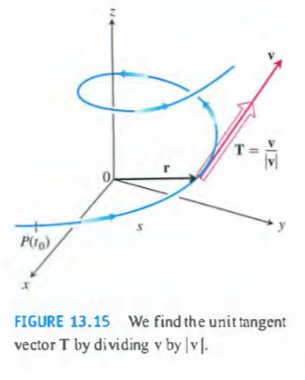
\includegraphics[scale=0.7]{m1_f28}
\end{center}

\bigskip

\hrulefill

\bigskip

\begin{example}
Calculate the distance along the curve $\bm{r}(t) = (\cos(t))\bm{i} + (\sin(t))\bm{j} + t\bm{k}$ between the points $P(1,0,0)$ and $Q(0,1,\pi/2)$.\\

\smallskip

If we think of $P$ as our base point and note that $P$ corresponds to $t=0$, we see that we want to calculate the integral
\begin{align*}
s(\pi/2) &= \int_0^{\pi/2} \sqrt{(-\sin(t))^2+(\cos(t))^2+1^2}dt\\
&= \int_0^{\pi/2} \sqrt{2}dt = \frac{\pi}{2} \sqrt{2}.
\end{align*}
\end{example}

\bigskip

\hrulefill

\bigskip

\begin{definition}
The \textbf{unit tangent vector} to a smooth curve is given by
\begin{align*}
\bm{T} = \frac{\bm{v}}{||\bm{v}||}.
\end{align*}
\end{definition}

\bigskip

\begin{center}
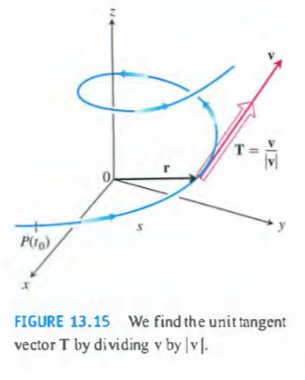
\includegraphics[scale=0.7]{m1_f28}
\end{center}

\bigskip

Noting that $\frac{ds}{dt} = ||\bm{v}(t)||$ by the FTOC, we could also write this as
\begin{align*}
\bm{T} &= \frac{\bm{v}}{||\bm{v}||}\\
&= \bm{v} \frac{1}{||\bm{v}||}\\
&= \frac{d\bm{r}}{dt} \frac{dt}{ds}\\
&= \frac{d\bm{r}}{ds}.
\end{align*}
Again, this will be useful later.

\bigskip

\hrulefill

\bigskip

\begin{example}
Find the unit tangent vector of the following curves.\\
\begin{itemize}
\item[1.] $\bm{r}(t) = (3\cos(t))\bm{i}+(3\sin(t))\bm{j}+t^2\bm{k}$
\begin{align*}
\bm{T} &= \frac{\bm{v}}{||\bm{v}||}\\
&= \frac{(-3\sin(t))\bm{i}+(3\cos(t))\bm{j}+2t\bm{k}}{\sqrt{9\sin^2(t)+9\cos^2(t)+4t^2}}\\
&= -\frac{3\sin(t)}{\sqrt{9+4t^2}}\bm{i}+\frac{3\cos(t)}{\sqrt{9+4t^2}}\bm{j}+\frac{2t}{\sqrt{9+4t^2}}\bm{k}
\end{align*}
\item[2.] $\bm{r}(t) = \langle t,t^2,t^3 \rangle$
\begin{align*}
\bm{T} &= \frac{\bm{v}}{||\bm{v}||}\\
&= \frac{\langle 1, 2t, 3t^2 \rangle}{\sqrt{1+4t^2+9t^4}}\\
&= \frac{1}{\sqrt{1+4t^2+9t^4}}\bm{i}+\frac{2t}{\sqrt{1+4t^2+9t^4}}\bm{j}+\frac{3t^2}{\sqrt{1+4t^2+9t^4}}\bm{k}
\end{align*}
\end{itemize}
\end{example}

\newpage

% --------------------------------------------------------------
%                         Sec 13.4
% --------------------------------------------------------------

\section{Curvature and Normal Vectors of a Curve (13.14)}

We would like to obtain some idea of ``how much" a curve turns or bends. We will do this by focusing on the unit tangent vector that we defined in the last section. Notice that if the unit tangent vector is not changing as we move along the curve (increase or decrease $s$), the curve cannot be curving. Continuing with this argument, we see that if the unit tangent vector is changing dramatically over some period of the curve then this mean the curve is turning or bending a lot. This leads to the following definition.

\bigskip

\begin{center}
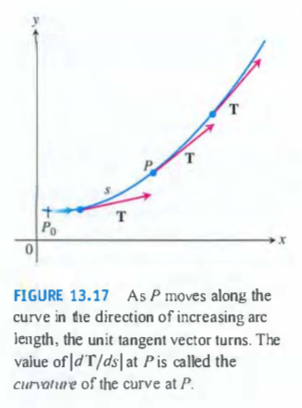
\includegraphics[scale=0.7]{m1_f30}
\end{center}

\bigskip

\begin{definition}
If $\bm{T}$ is the unit tangent vector of a smooth curve, the \textbf{curvature} function of the curve is
\begin{align*}
\kappa = \norm{\frac{d\bm{T}}{ds}}
\end{align*}
\end{definition}

\bigskip

Typically we are given $\bm{r}$ in terms of $t$, so we would like to find a formula for curvature in terms of $t$ instead. Note that
\begin{align*}
\kappa = \norm{\frac{d\bm{T}}{ds}} &= \norm{\frac{d\bm{T}}{dt} \frac{dt}{ds}}\\
&= \frac{1}{||ds/dt||} \norm{\frac{d\bm{T}}{dt}}\\
&= \frac{1}{||\bm{v}||}\norm{\frac{d\bm{T}}{dt}}.
\end{align*}
This is how you could calculate curvature in practice, but we won't typically need to do that in this class.

\bigskip

\hrulefill

\bigskip

We'll now introduce another important unit vector which is orthogonal to the unit tangent vector $\bm{T}$ at every point on the curve. Notice that if we can find this unit vector, it will always point in the direction that $\bm{T}$ is turning. It can be shown (left as an exercise) that for any vector $\bm{v}(t)$ of constant length we have
\begin{align*}
\bm{v} \cdot \frac{d\bm{v}}{dt} = 0.
\end{align*}
Thus we have
\begin{align*}
\bm{T} \cdot \frac{d\bm{T}}{ds} = 0,
\end{align*}
meaning $\frac{d\bm{T}}{ds}$ is orthogonal to $\bm{T}$. Therefore dividing $\frac{d\bm{T}}{ds}$ by its length will give us a unit vector that is orthogonal to $\bm{T}$ at every point on the curve.

\bigskip

\begin{definition}
At a point where $\kappa \neq 0$, the \textbf{principal unit normal} vector for a smooth curve in the plane is
\begin{align*}
\bm{N} &= \frac{\frac{d\bm{T}}{ds}}{\norm{\frac{d\bm{T}}{ds}}}\\
&= \frac{1}{\kappa} \frac{d\bm{T}}{ds}.
\end{align*}
\end{definition}

\bigskip

\begin{center}
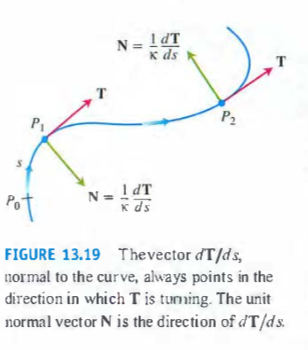
\includegraphics[scale=0.7]{m1_f31}
\end{center}

\bigskip

Again we would like to express this independently of $s$, so note that
\begin{align*}
\bm{N} &= \frac{\frac{d\bm{T}}{ds}}{\norm{\frac{d\bm{T}}{ds}}}\\
&= \frac{(d\bm{T}/dt)(dt/ds)}{||d\bm{T}/dt|| ||dt/ds||}\\
&= \frac{d\bm{T}/dt}{||d\bm{T}/dt||} \ \text{since} \ dt/ds>0.
\end{align*}

\bigskip

\hrulefill

\bigskip

\begin{example}
Find $\bm{N}$ for the circular motion $\bm{r}(t) = (\cos(2t)\bm{i}+(\sin(2t))\bm{j}$.\\

\smallskip

In order to use our formula we must find $\bm{T}$, which is given by
\begin{align*}
\bm{T} &= \frac{\bm{v}}{||\bm{v}||}\\
&= \frac{-(2\sin(2t))\bm{i}+(2\cos(2t))\bm{j}}{\sqrt{4\sin^2(2t)+4\cos^2(2t)}}\\
&= \frac{-(2\sin(2t))\bm{i}+(2\cos(2t))\bm{j}}{2}\\
&= -(\sin(2t))\bm{i} + (\cos(2t))\bm{j}.
\end{align*}
Now we have
\begin{align*}
\bm{N} &= \frac{d\bm{T}/dt}{||d\bm{T}/dt||}\\
&= \frac{-(2\cos(2t))\bm{i} -(2\sin(2t))\bm{j}}{\sqrt{4\cos^2(2t)+4\sin^2(2t)}}\\
&= \frac{-(2\cos(2t))\bm{i} -(2\sin(2t))\bm{j}}{2}\\
&= -(\cos(2t))\bm{i} -(\sin(2t))\bm{j}.
\end{align*}
Notice that $\bm{T}\cdot\bm{N} =0$ and that $\bm{N}$ points from $\bm{r}(t)$ towards the circle's center.
\end{example}

\bigskip

\hrulefill

\bigskip

\begin{example}
Find $\bm{N}$ for the helix $\bm{r}(t) = \langle \cos(t), \sin(t), t \rangle$. \\

\smallskip

Here we have
\begin{align*}
\bm{T} &= \frac{\bm{v}}{||\bm{v}||}\\
&= \frac{\langle -\sin(t), \cos(t), 1 \rangle}{\sqrt{\sin^2(t)+\cos^2(t)+1^2}}\\
&= \frac{\langle -\sin(t), \cos(t), 1 \rangle}{\sqrt{2}}\\
&= \bigg\langle -\frac{\sin(t)}{\sqrt{2}}, \frac{\cos(t)}{\sqrt{2}}, \frac{1}{\sqrt{2}} \bigg\rangle.
\end{align*}
Which gives
\begin{align*}
\bm{N} &= \frac{d\bm{T}/dt}{||d\bm{T}/dt||}\\
&= \frac{\bigg\langle -\frac{\cos(t)}{\sqrt{2}}, -\frac{\sin(t)}{\sqrt{2}}, 0 \bigg\rangle}{\sqrt{\frac{\cos^2(t)}{2}+\frac{\sin^2(t)}{2}}}\\
&= \bigg\langle -\cos(t), -\sin(t), 0 \bigg\rangle.
\end{align*}
\end{example}

\newpage

% --------------------------------------------------------------
%                         Sec 13.5
% --------------------------------------------------------------

\section{Tangential and Normal Components of Acceleration (13.5)}

The three dimensional coordinate system we have learned about is often ``good enough" to describe the position, velocity, and acceleration of a particle in space. But is it possible to define a new coordinate system that better and more easily describes the movement of a particle along a space curve? The answer is yes! We need three vectors to define this coordinate system, and we already know two of them. Let's look at the third.

\bigskip

\begin{definition}
The \textbf{binormal vector} of a curve in space is $\bm{B} = \bm{T} \times \bm{N}$, a unit vector orthogonal to both $\bm{T}$ and $\bm{N}$. Together $\bm{T}$, $\bm{N}$ and $\bm{B}$ define a moving right-handed vector frame known as the \textbf{Frenet frame} or more commonly as the \textbf{TNB frame}.
\end{definition}

\bigskip

\hrulefill

\bigskip

I would recommend showing the animation at http://tinyurl.com/qexokbv to help students visualize the TNB frame. Now that we have this coordinate system, let's take a look at how we can rewrite the acceleration of a particle in terms of the TNB frame.

\bigskip

First see that
\begin{align*}
\bm{v} = \frac{d\bm{r}}{dt} = \frac{d\bm{r}}{ds}\frac{ds}{dt} = \bm{T} \frac{ds}{dt}.
\end{align*}
Now differentiating this we get
\begin{align*}
\bm{a} &= \frac{d\bm{v}}{dt} = \frac{d}{dt} \left(\bm{T} \frac{ds}{dt}\right) = \frac{d^2s}{dt^2} \bm{T} + \frac{ds}{dt} \frac{d\bm{T}}{dt}\\
&= \frac{d^2s}{dt^2} \bm{T} + \frac{ds}{dt} \left(\frac{d\bm{T}}{ds} \frac{ds}{dt}\right) = \frac{d^2s}{dt^2} \bm{T} + \frac{ds}{dt}\left(\kappa \bm{N} \frac{ds}{dt}\right)\\
&= \frac{d^2s}{dt^2} \bm{T} + \kappa \left(\frac{ds}{dt}\right)^2 \bm{N}.
\end{align*}

\bigskip

This leads to the following definition.

\bigskip

\begin{definition}
If the acceleration vector is written as
\begin{align*}
\bm{a} = a_T \bm{T} + a_N \bm{N},
\end{align*}
then
\begin{align*}
a_T = \frac{d^2s}{dt^2} = \frac{d}{dt}||\bm{v}|| \ \ \text{and} \ \ a_N = \kappa \left(\frac{ds}{dt}\right)^2 = \kappa ||\bm{v}||^2
\end{align*}
are the \textbf{tangential} and \textbf{normal} scalar components of acceleration.
\end{definition}

\bigskip

\textbf{Notes:}
\begin{itemize}
\item Notice that the vector $\bm{B}$ is not present in the above definition. That means the acceleration vector $\bm{a}$ always lies in the plane given by of $\bm{T}$ and $\bm{N}$. This also means that $\bm{a}$ is always orthogonal to $\bm{B}$!
\item With the above definition, we can see that the acceleration component $a_T$ measures the rate of change of the \textit{length} of $\bm{v}$, while $a_N$ measures the rate of change of the \textit{direction} of $\bm{v}$.
\item Potentially useful formulas are as follows:
\begin{align*}
a_T = \bm{a} \cdot \bm{T} \ \ \text{and} \ \ a_N = \bm{a} \cdot \bm{N}.
\end{align*}
\end{itemize}

\bigskip

\hrulefill

\bigskip

\begin{example}
Find $\bm{a}$ in terms of $\bm{T}$ and $\bm{N}$ for the helix $\bm{r} = \langle \cos(t),\sin(t), t\rangle$.

\smallskip

We have already see that $\bm{T} = \bigg\langle -\frac{\sin(t)}{\sqrt{2}}, \frac{\cos(t)}{\sqrt{2}}, \frac{1}{\sqrt{2}} \bigg\rangle$ and $\bm{N} = \bigg\langle -\cos(t), -\sin(t), 0 \bigg\rangle$. We've also seen that $\bm{a}(t) = \langle -\cos(t), -\sin(t), 0 \rangle$, so we know that
\begin{align*}
a_T = \bm{a} \cdot \bm{T} &= \langle -\cos(t), -\sin(t), 0 \rangle \cdot \bigg\langle -\frac{\sin(t)}{\sqrt{2}}, \frac{\cos(t)}{\sqrt{2}}, \frac{1}{\sqrt{2}} \bigg\rangle\\
&= \frac{\cos(t)\sin(t)}{\sqrt{2}} -\frac{\cos(t)\sin(t)}{\sqrt{2}}\\
&= 0.
\end{align*}
and
\begin{align*}
a_N = \bm{a}\cdot\bm{N} &=  \langle -\cos(t), -\sin(t), 0 \rangle \cdot \bigg\langle -\cos(t), -\sin(t), 0 \bigg\rangle\\
&=\cos^2(t)+\sin^2(t)\\
&=1.
\end{align*}
Thus we have
\begin{align*}
\bm{a} = a_T \bm{T} + a_N \bm{N} &= 1\bm{N}\\
\end{align*}
\end{example}

\end{document}